\begin{figure*}
    \centering
    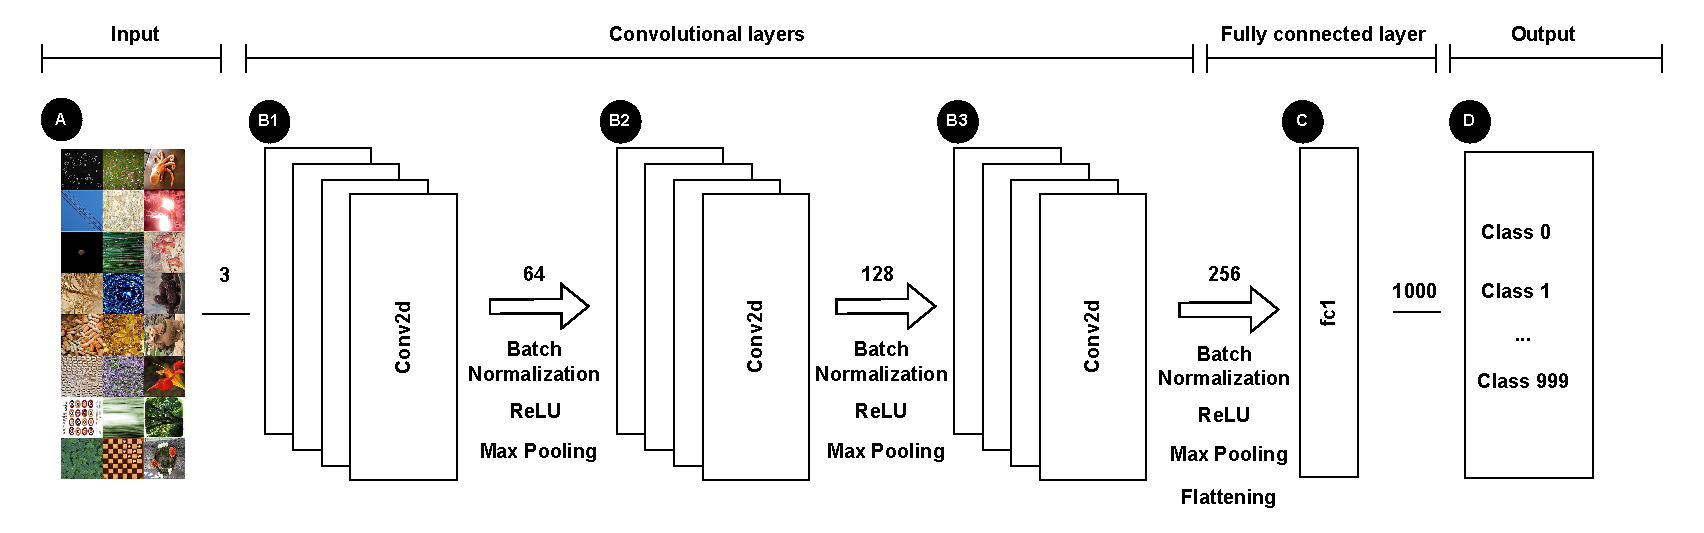
\includegraphics[width=0.95\linewidth]{figures/SiMo-overview.pdf}
    \caption{A high-level architectural overview of SiMo, a simple architectural model.}
    \label{fig:design:f3}\label{fig:design:simo}
\end{figure*}


\section{Background } \label{sec:background}

Object detection is one of the core problems in computer vision, which involves identifying key features of certain structures. Any other computer vision task inherently bases itself on the same number of methods as a basic object detection task. It therefore a prerequisite for other computer vision challenges, making it essential in domains such as autonomous vehicles \cite{DBLP:conf/cvpr/GeigerLU12}, medical imaging \cite{LITJENS201760}, or geospatial analysis \cite{9676295}.

To have an accurate object detection, we need a model that analyses both local and global features of an image \cite{DBLP:conf/clor/MurphyTEF06}. Local features, such as edges and corners, are essential for distinguishing fine-grained details, especially in cases where objects have slight differences. However, global features provide a broader contextual understanding of the entire image, which helps recognize objects based on their spatial relationships.

Given that our main goal with this paper is to explore the trade-off between model complexity and performance, EfficientNet serves as an excellent candidate for our complex model.

While traditional convolutional neural networks effectively detect local patterns, their subcategory, EfficientNet, is a superior choice for high-accuracy object detection tasks \cite{tan_efficientnet_2020}.

EfficientNet is a family of CNNs designed to maximize accuracy and minimize computational cost \cite{DBLP:conf/cvpr/TanPL20}. Unlike traditional CNNs, EfficientNet employs a compound coefficient that is used to uniformly scale all dimensions of width, depth, and resolution. This allows it to incorporate more global information about the image. EfficientNet models are labeled B0 to B7, with B0 being the smallest and most computationally efficient, and B7 offering the highest accuracy at the expense of increased complexity.

For training and testing of our models, we used ImageNet-1K, a large-scale dataset widely used for training and benchmarking deep learning models in image classification tasks~\cite{DBLP:conf/cvpr/DengDSLL009}. ImageNet-1k consists of over a million images across 1,000 classes. Many state-of-the-art models, including EfficientNet, have been benchmarked on ImageNet-1K, making it a relevant choice for our study~\cite{DBLP:conf/icml/TanL19}. We decided on ImageNet-1K because of its diversity, size, and widespread adoption, which would ensure robust model evaluation~\cite{DBLP:journals/cacm/KrizhevskySH17}.

% suggested for background:
% 1. talk more about efficientNets, why are they useful, why did we choose them
% 2. talk a bit about ImageNet 1k, where it was used
% for 1, 2, would be nice to give some literature and references
% mention some metrics which we are using for measuring accuracy 
% you can go up to 1/4 of the second column of the page and save a bit by making a small(er) F2 figure
